\chapter{Velocidad de grupo, exclusión fermiónica y mar de Dirac}

\section{Velocidad de fase y velocidad de grupo}

\begin{classroomqa}\lecturetimestamp{00:00:07}\audiencequestion{¿Qué son la velocidad de grupo y la velocidad de fase?}\lecturerresponse{La velocidad de fase sigue un punto de fase constante de una onda plana. En general, no describe el movimiento de un objeto medible. La velocidad de grupo sigue la envolvente de un paquete de ondas y es la velocidad asociada a las partículas, las señales y el flujo de probabilidad.}\end{classroomqa}

Partamos de una onda plana,
\begin{equation}
\psi(x,t)=e^{i(kx-\omega t)},
\end{equation}
o de su forma real,
\begin{equation}
\psi(x,t)=\sin(kx-\omega t).
\end{equation}
Una cresta, un valle o cualquier otro punto de fase constante se mueve de modo que
\begin{equation}
kx-\omega t=\text{constant}.
\end{equation}
Por comodidad, elijamos que la constante sea cero. Así obtenemos
\begin{equation}
x=\frac{\omega}{k}t,
\qquad
v_{\mathrm{phase}}=\frac{\omega}{k}.
\end{equation}
Como \(\omega=2\pi/T\) y \(k=2\pi/\lambda\),
\begin{equation}
v_{\mathrm{phase}}=\frac{\omega}{k}=\frac{\lambda}{T}.
\end{equation}
Esto es simplemente la distancia que avanza una fase dada durante un período.

Para una onda Schr\"odinger no relativista, con \(\hbar=1\), la energía y el momento son \(\omega\) y \(k\), respectivamente, de modo que
\begin{equation}
\omega(k)=\frac{k^2}{2m}.
\end{equation}
Por tanto, su velocidad de fase es
\begin{equation}
v_{\mathrm{phase}}=\frac{k}{2m}.
\end{equation}
Sin embargo, la velocidad ordinaria de una partícula con momento \(k\) es \(k/m\). Esta discrepancia por un factor de dos es la primera advertencia de que el movimiento de la fase de una onda plana no es el movimiento de la partícula.

Hay una advertencia aún más clara. Sumemos la misma constante \(C\) a todas las frecuencias:
\begin{equation}
\omega(k)\longrightarrow \omega(k)+C.
\end{equation}
Por ejemplo, la constante podría representar una contribución común de energía en reposo, como \(mc_{\mathrm{light}}^2\), pero su nombre concreto no es importante. Aquí \(C\) es un desplazamiento de energía, no la velocidad de la luz. La velocidad de fase cambia a
\begin{equation}
v_{\mathrm{phase}}\longrightarrow
\frac{\omega(k)+C}{k}
=v_{\mathrm{phase}}+\frac{C}{k}.
\end{equation}
Sin embargo, sumar la misma constante a todas las energías no cambia ninguna diferencia de energía y, por tanto, tampoco cambia la física no relativista.

Esto se ve directamente en la función de onda. Escribamos un campo Schr\"odinger general como una suma o integral de modos,
\begin{equation}
\psi(x,t)=\sum_k a_k e^{ikx}e^{-i\omega(k)t},
\end{equation}
sin incluir los factores de normalización. Después del desplazamiento,
\begin{align}
\psi(x,t)
&\longrightarrow
\sum_k a_k e^{ikx}e^{-i[\omega(k)+C]t}
\\
&=e^{-iCt}\psi(x,t).
\end{align}
Todos los modos han adquirido la misma fase dependiente del tiempo. El campo conjugado adquiere la fase opuesta, por lo que
\begin{equation}
\begin{aligned}
\psi^*(x,t)\psi(x,t)
&\longrightarrow
e^{iCt}e^{-iCt}\psi^*(x,t)\psi(x,t)
\\
&=\psi^*(x,t)\psi(x,t).
\end{aligned}
\end{equation}
La misma cancelación se produce en los valores esperados. Una cantidad que cambia al desplazar el cero de energía no puede ser la velocidad física de propagación de la partícula Schr\"odinger. Por tanto, la velocidad de fase es en parte convencional.

Una partícula localizada no se representa mediante una sola onda plana infinita, sino mediante un paquete. Las ondas componentes se suman constructivamente en la región del paquete y destructivamente fuera de ella. El movimiento de este patrón puede obtenerse a partir de dos ondas próximas:
\begin{equation}
\psi(x,t)=
\sin(kx-\omega t)+
\sin(k'x-\omega't),
\end{equation}
donde \(k'\) está cerca de \(k\) y \(\omega'=\omega(k')\). Hay interferencia constructiva en los puntos donde sus fases coinciden:
\begin{equation}
kx-\omega t=k'x-\omega't.
\end{equation}
Por tanto,
\begin{equation}
(k-k')x=(\omega-\omega')t,
\end{equation}
y el patrón de refuerzo se mueve según
\begin{equation}
x=\frac{\omega-\omega'}{k-k'}t.
\end{equation}
Al tomar el límite de ondas vecinas se obtiene
\begin{equation}
x=\frac{d\omega}{dk}t,
\qquad
v_{\mathrm{group}}=\frac{d\omega}{dk}.
\end{equation}
Esta es la velocidad de la envolvente---, el bulto localizado producido por la interferencia de las ondas componentes.

Para la relación de dispersión no relativista, incluido el desplazamiento arbitrario,
\begin{equation}
\omega(k)=\frac{k^2}{2m}+C,
\end{equation}
la velocidad de grupo es
\begin{equation}
v_{\mathrm{group}}
=\frac{d}{dk}\left(\frac{k^2}{2m}+C\right)
=\frac{2k}{2m}
=\frac{k}{m}.
\end{equation}
La constante aditiva ha desaparecido y el resultado es precisamente la velocidad clásica de la partícula.

\begin{classroomqa}\lecturetimestamp{00:16:35}\audiencequestion{¿Desaparece el factor de dos en la velocidad de grupo?}\lecturerresponse{Sí. Al derivar \(k^2\) se obtiene \(2k\), que cancela el dos de \(2m\). El resultado es \(k/m\).}\end{classroomqa}

Por consiguiente, la velocidad de grupo es la que se asocia más estrechamente con el movimiento clásico de las partículas. También es la velocidad pertinente para la propagación de un paquete y, en las circunstancias ordinarias que consideramos aquí, para la propagación de señales. La velocidad de fase no tiene por qué tener ninguno de esos significados.

\subsection{Ondas relativistas con masa y sin masa}

\begin{classroomqa}\lecturetimestamp{00:17:47}\audiencequestion{¿Tiene esto que ver con las afirmaciones de que la luz puede viajar más rápido que la luz?}\lecturerresponse{No. Esas afirmaciones plantean otra cuestión. Un cálculo relacionado sí muestra que una fase puede moverse más rápido que la luz mientras la velocidad de grupo física sigue siendo sublumínica, pero eso no describe una señal que adelante a la luz.}\end{classroomqa}

\begin{classroomqa}\lecturetimestamp{00:18:05}\audiencequestion{¿El ejemplo pertinente es el conocido caso en que la velocidad de fase supera la velocidad de la luz mientras que la velocidad de grupo permanece por debajo?}\lecturerresponse{Sí. El mismo patrón aparece en una onda relativista con masa distinta de cero, y se deduce directamente de la relación entre la energía--y el momento relativistas.}\end{classroomqa}

Tomemos \(\hbar=c_{\mathrm{light}}=1\). La relación relativista es
\begin{equation}
E=\sqrt{p^2+m^2},
\qquad
\omega(k)=\sqrt{k^2+m^2}.
\end{equation}
Conviene establecer primero el caso sin masa. Cuando \(m=0\),
\begin{equation}
\omega=|k|.
\end{equation}
En la rama que se propaga hacia la derecha, \(k>0\), \(\omega=k\) y, por tanto,
\begin{equation}
v_{\mathrm{phase}}=\frac{\omega}{k}=1,
\qquad
v_{\mathrm{group}}=\frac{d\omega}{dk}=1.
\end{equation}
En la rama que se propaga hacia la izquierda, ambas velocidades tienen el signo negativo correspondiente. En cualquiera de los dos casos, su módulo es la velocidad de la luz. Como la relación de dispersión es lineal en cada rama, todas las componentes de Fourier de esa rama se mueven con la misma velocidad.

Para una partícula con masa y \(k>0\),
\begin{equation}
v_{\mathrm{phase}}
=\frac{\omega}{k}
=\sqrt{\frac{k^2+m^2}{k^2}}>1,
\end{equation}
mientras que
\begin{equation}
v_{\mathrm{group}}
=\frac{d\omega}{dk}
=\frac{k}{\sqrt{k^2+m^2}}<1.
\end{equation}
Para \(k<0\), ambas velocidades cambian de signo, pero sus módulos obedecen las mismas desigualdades. Así, la fase puede moverse más rápido que la luz mientras que el paquete, la partícula, la energía y la señal se mueven más despacio que la luz. Para esta relación de dispersión particular y \(k\neq0\),
\begin{equation}
v_{\mathrm{phase}}v_{\mathrm{group}}=1.
\end{equation}
Esa relación inversa es una particularidad de la relación de dispersión de raíz cuadrada, no una propiedad general de las ondas.

\begin{figure}\centering
\includegraphics[width=0.72\textwidth]{lecture_05_figure_03.png}\caption{Relaciones de dispersión no relativista y relativista, con velocidad de fase \(\omega/k\) y velocidad de grupo \(d\omega/dk\).}\lectureframe{00:35:52}\end{figure}

\begin{classroomqa}\lecturetimestamp{00:23:41}\audiencequestion{¿La dispersión está relacionada con que la velocidad de onda dependa de la frecuencia?}\lecturerresponse{Sí. Cuando \(\omega(k)\) es lineal, todas las componentes de Fourier tienen la misma velocidad de grupo y el paquete puede conservar su forma. Cuando \(\omega(k)\) es no lineal, las distintas componentes se mueven a velocidades diferentes, por lo que el paquete se dispersa y cambia de forma. El sonido de baja frecuencia es aproximadamente no dispersivo cuando su frecuencia es casi proporcional al número de onda.}\end{classroomqa}

En general, la velocidad de fase no transporta señales, energía ni flujo de probabilidad. Su valor numérico incluso puede cambiarse al desplazar el cero de energía. La velocidad de grupo describe el movimiento físicamente pertinente de un paquete suficientemente estrecho.

\begin{classroomqa}\lecturetimestamp{00:25:14}\audiencequestion{¿Se puede medir la velocidad de fase de un fotón?}\lecturerresponse{En el vacío, un fotón tiene una relación de dispersión lineal, por lo que sus velocidades de fase y de grupo coinciden y ambas son iguales a la velocidad de la luz. En un medio material cambia la relación de dispersión, y las velocidades de fase y de grupo pueden diferir.}\end{classroomqa}

\begin{classroomqa}\lecturetimestamp{00:25:50}\audiencequestion{¿Esta discusión se limita a los paquetes de ondas que no se ensanchan con el tiempo?}\lecturerresponse{Un paquete solo permanece sin ensancharse cuando todas sus componentes de Fourier comparten una misma velocidad, lo que corresponde a una relación de dispersión lineal en el intervalo pertinente. Con una dispersión no lineal, las componentes se separan y el paquete se ensancha.}\end{classroomqa}

Las cuestiones sobre los conos de luz y la estructura causal relativista requieren algo más que distinguir entre velocidad de fase y velocidad de grupo, por lo que se tratan aparte de este cálculo.

\section{Simetría de traslación y leyes de conservación}

Las mismas fases de las ondas planas permiten describir las leyes de conservación de forma concisa. Empecemos por la conservación de la energía. Un campo de aniquilación que actúa sobre una partícula entrante de energía \(\omega_j\) aporta un factor temporal
\begin{equation}
e^{-i\omega_j t},
\end{equation}
mientras que un campo de creación que produce una partícula saliente de energía \(\omega'_r\) aporta
\begin{equation}
e^{+i\omega'_r t}.
\end{equation}
Para varias partículas entrantes y salientes, el producto de esos factores es
\begin{equation}
\exp\!\left[
i\left(\sum_r\omega'_r-\sum_j\omega_j\right)t
\right].
\end{equation}
Si la interacción puede ocurrir en cualquier instante con la misma amplitud, la amplitud incluye una integral sobre el tiempo de interacción:
\begin{equation}
\begin{aligned}
&\int_{-\infty}^{\infty}dt\,
\exp\!\left[
i\left(\sum_r\omega'_r-\sum_j\omega_j\right)t
\right]
\\
&\quad =2\pi\,
\delta\!\left(\sum_r\omega'_r-\sum_j\omega_j\right).
\end{aligned}
\end{equation}
La función delta exige que la energía total saliente sea igual a la energía total entrante. Que la amplitud sea la misma en todo instante posible de interacción expresa la invariancia ante traslaciones temporales y da lugar a la conservación de la energía.

Las traslaciones espaciales dan lugar a la conservación del momento mediante el mismo mecanismo. Consideremos un decaimiento físico de una partícula en dos, en el que desaparece una partícula entrante de momento \(k\) y aparecen dos partículas de momentos \(k'_1\) y \(k'_2\). Una interacción local en la posición \(x\) contiene un campo de aniquilación y dos campos de creación:
\begin{equation}
\mathcal{O}(x)=\psi^\dagger(x)\psi^\dagger(x)\psi(x).
\end{equation}
Omitiendo la dependencia temporal y la normalización, los factores de modo pertinentes son
\begin{align}
\psi(x)&\supset a_k e^{ikx},
\\
\psi^\dagger(x)&\supset a_{k'_1}^\dagger e^{-ik'_1x},
\qquad
\psi^\dagger(x)\supset a_{k'_2}^\dagger e^{-ik'_2x}.
\end{align}
En el elemento de matriz
\begin{equation}
\langle k'_1,k'_2|\mathcal{O}(x)|k\rangle,
\end{equation}
el operador de aniquilación elimina la partícula entrante y los dos operadores de creación aportan las partículas salientes. Una vez realizadas esas acciones de los operadores, queda el siguiente factor dependiente de la posición:
\begin{equation}
e^{-ik'_1x}e^{-ik'_2x}e^{ikx}
=e^{i(k-k'_1-k'_2)x}.
\end{equation}
Como ninguna posición es privilegiada, se integra sobre todas las posiciones posibles del decaimiento:
\begin{equation}
\int_{-\infty}^{\infty}dx\,
e^{i(k-k'_1-k'_2)x}
=2\pi\delta(k-k'_1-k'_2).
\end{equation}
Por tanto, la amplitud resultante satisface
\begin{equation}
k=k'_1+k'_2.
\end{equation}
En tres dimensiones, el mismo cálculo usa \(d^3x\), vectores de momento en negrita y una función delta tridimensional. El argumento no depende de que haya una sola partícula entrante o dos salientes. Para un número arbitrario de partículas, la integración sobre la posición común de interacción produce
\begin{equation}
\delta^{(3)}\!\left(
\sum_j\mathbf{k}_j-\sum_r\mathbf{k}'_r
\right).
\end{equation}
Que la amplitud sea la misma en todas las posiciones expresa la invariancia ante traslaciones espaciales y da lugar a la conservación del momento, del mismo modo que una amplitud igual en todo instante da lugar a la conservación de la energía.

Un tercer ejemplo es una rotación global de fase:
\begin{equation}
\psi\longrightarrow e^{i\lambda}\psi,
\qquad
\psi^\dagger\longrightarrow e^{-i\lambda}\psi^\dagger.
\end{equation}
La amplitud de interacción es invariante cuando se cancelan las fases aportadas por sus campos de aniquilación y de creación. Para un campo con carga eléctrica, esta igualdad entre la carga retirada del estado inicial y la restituida en el estado final expresa la conservación de la carga. Así, las traslaciones temporales, las traslaciones espaciales y las rotaciones globales de fase ilustran cómo los campos que crean y aniquilan partículas codifican la conservación de la energía, el momento y la carga.

\begin{classroomqa}\lecturetimestamp{00:37:52}\audiencequestion{¿La integración sobre el espacio abarca las tres dimensiones espaciales?}\lecturerresponse{Sí. Las tres integraciones producen una función delta para las tres componentes del momento, por lo que se conservan las tres componentes del momento total.}\end{classroomqa}

\begin{classroomqa}\lecturetimestamp{00:38:03}\audiencequestion{¿Este modelo determina las probabilidades relativas de las distintas maneras de repartir el momento conservado?}\lecturerresponse{No. Esta expresión sencilla impone la suma de los momentos salientes, pero no determina cómo se reparten. Para hallar las probabilidades relativas se necesita información dinámica adicional.}\end{classroomqa}

\begin{classroomqa}\lecturetimestamp{00:39:04}\audiencequestion{¿Por qué una suma de operadores de aniquilación se reduce al término correspondiente al momento ocupado?}\lecturerresponse{Un operador de aniquilación aplicado a un modo vacío da el vector nulo. Si el estado contiene una sola partícula, únicamente en el modo \(k_0\), todos los términos salvo el que tiene \(k=k_0\) se anulan.}\end{classroomqa}

Por ejemplo,
\begin{equation}
\sum_k a_k e^{ikx}|1_{k_0}\rangle
=e^{ik_0x}|0\rangle,
\end{equation}
salvo por la normalización: todos los operadores de aniquilación asociados a modos vacíos devuelven el vector nulo.

\section{Realce bosónico y exclusión fermiónica}

Los bosones admiten cualquier número de ocupación no negativo en un estado de una partícula, y el álgebra de sus operadores de creación favorece, de hecho, un estado ya ocupado. Para un modo bosónico, la convención de estados de número normalizados expresa el realce de la ocupación como\footnote{La clase indica el realce de la ocupación por la raíz cuadrada; esta ecuación indexada presenta su forma estándar en estados de número.}\begin{equation}
a^\dagger|n\rangle=\sqrt{n+1}\,|n+1\rangle.
\end{equation}
Supongamos que un átomo excitado puede emitir un fotón en muchos modos posibles. Si no hay otros fotones, las distintas direcciones y momentos aparecen con su distribución de probabilidad habitual. Si un modo concreto ya contiene muchos fotones---todos con el mismo momento, energía y frecuencia---, la emisión en ese modo se ve realzada por el factor correspondiente de raíz cuadrada de la ocupación. El átomo tiende a añadir su fotón al estado que ya está poblado. Esta es la emisión estimulada y constituye una manifestación concreta de la congregación bosónica.

Los fermiones se comportan de manera opuesta. Dos fermiones idénticos no pueden ocupar el mismo estado cuántico. El principio de exclusión surgió primero en la física atómica, donde dos electrones de un átomo no pueden tener números cuánticos idénticos, pero no se limita a los átomos: los fermiones idénticos no pueden compartir un estado completo de una partícula en ningún lugar.

Al principio, la expansión del campo parece igual que la de los bosones. En una caja finita se puede escribir
\begin{equation}
\psi(x)=\sum_k A_k e^{ikx},
\qquad
\psi^\dagger(x)=\sum_k A_k^\dagger e^{-ikx}.
\end{equation}
Para momentos continuos, las sumas se convierten en integrales. El signo opuesto en la fase espacial conjugada se debe a la conjugación hermítica. Esta parte de la construcción es no relativista; los fermiones relativistas aparecerán solo al final.

El estado del campo sigue especificándose mediante un número de ocupación para cada modo, pero ahora cada número solo puede ser cero o uno:
\begin{equation}
|n_{k_1},n_{k_2},\ldots\rangle,
\qquad n_k\in\{0,1\}.
\end{equation}
No existen otros tipos de partículas relativistas que, por ejemplo, permitan como máximo tres partículas por estado o exijan al menos siete. Demostrar que las estadísticas bosónicas y fermiónicas son las únicas posibilidades requiere la mecánica cuántica junto con la relatividad especial y queda fuera del alcance de esta discusión. Aquí la tarea consiste en describir la posibilidad fermiónica y sus consecuencias.

\subsection{Un estado fermiónico}

Concentrémonos en un único estado de una partícula. Puede estar vacío, \(|0\rangle\), o ocupado, \(|1\rangle\). Los operadores de creación y aniquilación actúan así:
\begin{align}
A^\dagger|0\rangle&=|1\rangle,
&
A^\dagger|1\rangle&=0,
\\
A|0\rangle&=0,
&
A|1\rangle&=|0\rangle.
\end{align}
El cero sin adornos del lado derecho es el vector nulo, no el estado vacío \(|0\rangle\). Intentar añadir un segundo fermión no devuelve el vacío: no produce ningún estado físico.

\begin{classroomqa}\lecturetimestamp{00:46:25}\audiencequestion{¿Los operadores fermiónicos de creación y aniquilación siguen siendo lineales?}\lecturerresponse{Sí. Los operadores de la mecánica cuántica son operadores lineales, incluidos los operadores fermiónicos de creación y aniquilación.}\end{classroomqa}

\begin{classroomqa}\lecturetimestamp{00:47:34}\audiencequestion{¿El cero significa el estado vacío o significa que la operación intentada no puede producir un estado?}\lecturerresponse{Significa el vector nulo, no el estado vacío. El vacío verdadero o estado fundamental tiene una función de onda distinta de cero; la función idénticamente nula tiene norma cero y no es un estado físico.}\end{classroomqa}

El oscilador armónico permite ver la distinción con claridad. Su estado fundamental, el estado sin excitaciones del oscilador, tiene una función de onda gaussiana como
\begin{equation}
\phi_0(q)\propto e^{-\alpha q^2},
\qquad \alpha>0.
\end{equation}
Es un estado perfectamente válido y normalizable. En cambio,
\begin{equation}
\phi(q)\equiv0
\end{equation}
es el vector nulo: no tiene amplitud de probabilidad en ningún lugar y no es un estado. Así, \(A^\dagger|1\rangle=0\) indica que el segundo intento de creación produce el vector nulo.

\begin{classroomqa}\lecturetimestamp{00:48:42}\audiencequestion{¿Conviene usar una notación distinta para los operadores fermiónicos y bosónicos?}\lecturerresponse{Sí. Es más claro reservar \(a\) y \(a^\dagger\) para los modos bosónicos, y usar \(c\) y \(c^\dagger\) para los fermiónicos. En la bibliografía aparecen ambas convenciones, pero usar letras distintas permite distinguir las dos álgebras.}\end{classroomqa}

Con esa notación, las reglas para un solo modo son
\begin{align}
c^\dagger|0\rangle&=|1\rangle,
&c^\dagger|1\rangle&=0,
\\
c|0\rangle&=0,
&c|1\rangle&=|0\rangle.
\end{align}
Evaluemos ahora los dos productos posibles sobre los dos estados de la base. Para el estado vacío,
\begin{align}
c^\dagger c|0\rangle&=0,
&
cc^\dagger|0\rangle&=|0\rangle.
\end{align}
Para el estado ocupado,
\begin{align}
c^\dagger c|1\rangle&=|1\rangle,
&
cc^\dagger|1\rangle&=0.
\end{align}
La suma devuelve el estado sobre el que actúa:
\begin{align}
(c^\dagger c+cc^\dagger)|0\rangle&=|0\rangle,
\\
(c^\dagger c+cc^\dagger)|1\rangle&=|1\rangle.
\end{align}
Como \(|0\rangle\) y \(|1\rangle\) generan el espacio de estados de un modo,
\begin{equation}
c^\dagger c+cc^\dagger=1.
\end{equation}
La combinación con signo más es el anticonmutador,
\begin{equation}
\{A,B\}=AB+BA,
\end{equation}
por lo que la relación fermiónica es
\begin{equation}
\{c,c^\dagger\}=1.
\end{equation}
Es el análogo fermiónico del conmutador bosónico
\begin{equation}
[a,a^\dagger]=aa^\dagger-a^\dagger a=1.
\end{equation}

Dos operaciones de creación en el mismo estado fermiónico siempre se anulan. Si el estado está vacío, la primera creación lo ocupa y la segunda falla; si ya está ocupado, la primera creación ya falla. Del mismo modo, dos operaciones de aniquilación siempre se anulan. Por tanto,
\begin{equation}
\{c^\dagger,c^\dagger\}=2(c^\dagger)^2=0,
\qquad
\{c,c\}=2c^2=0.
\end{equation}

\begin{classroomqa}\lecturetimestamp{00:56:45}\audiencequestion{¿El cero en la relación del cuadrado del operador de aniquilación es un vector nulo?}\lecturerresponse{La ecuación afirma que \(c^2\) es el operador nulo. Es un operador que envía cualquier vector de estado al vector nulo. El operador nulo y el vector nulo son objetos matemáticos distintos, aunque el primero siempre produce el segundo.}\end{classroomqa}

Para muchos modos discretos de momento, el álgebra completa es
\begin{align}
\{c_k,c_{k'}^\dagger\}&=\delta_{kk'},
\\
\{c_k,c_{k'}\}&=0,
\\
\{c_k^\dagger,c_{k'}^\dagger\}&=0.
\end{align}
La delta de Kronecker vale uno cuando \(k=k'\) y cero en caso contrario. Para momentos continuos se reemplaza, con la normalización adecuada, por una delta de Dirac. Los anticonmutadores entre operadores del mismo tipo se anulan para cualquier par de modos, no solo cuando coinciden sus índices.

\subsection{Exclusión en el espacio de posiciones}

El álgebra etiquetada por el momento dice primero que dos fermiones idénticos de la misma especie no pueden ocupar un mismo modo de momento. Pero también dice algo más. Una partícula localizada en la posición \(x\) se crea mediante
\begin{equation}
\psi^\dagger(x)=\sum_k c_k^\dagger e^{-ikx},
\end{equation}
salvo por la normalización. En el origen, intentar crear dos partículas da
\begin{align}
\psi^\dagger(0)\psi^\dagger(0)|\Omega\rangle
&=\sum_{k,k'}c_k^\dagger c_{k'}^\dagger|\Omega\rangle.
\end{align}
Los índices \(k\) y \(k'\) son variables mudas de suma. Intercambiarlos no altera la suma doble, así que se puede promediar con la expresión en que se han intercambiado los índices:
\begin{align}
\sum_{k,k'}c_k^\dagger c_{k'}^\dagger|\Omega\rangle
&=\frac12\sum_{k,k'}
\left(c_k^\dagger c_{k'}^\dagger
+c_{k'}^\dagger c_k^\dagger\right)|\Omega\rangle
\\
&=\frac12\sum_{k,k'}
\{c_k^\dagger,c_{k'}^\dagger\}|\Omega\rangle
=0.
\end{align}

\begin{classroomqa}\lecturetimestamp{01:02:26}\audiencequestion{¿En la suma del estado de dos partículas en una posición solo se anulan los términos con momentos distintos?}\lecturerresponse{No. Al cambiar los índices mudos, toda la suma doble se convierte en la mitad del anticonmutador de dos operadores de creación. Ese anticonmutador se anula para cualquier par de momentos, así que la suma completa es cero.}\end{classroomqa}

El cálculo muestra que la exclusión no es exclusiva de los estados propios del momento. Tampoco se pueden colocar fermiones idénticos en un mismo estado de posición. En general, no pueden ocupar estados idénticos de una partícula.

\subsection{¿Qué significa que dos estados sean el mismo?}

\begin{classroomqa}\lecturetimestamp{01:04:30}\audiencequestion{¿Pueden dos electrones muy alejados tener el mismo momento?}\lecturerresponse{La exclusión se refiere al estado completo de una partícula. Dos electrones pueden tener el mismo valor propio exacto del momento si difieren en otra etiqueta que conmute con él, como el espín. En cambio, los electrones separados espacialmente son paquetes localizados, no estados propios exactos del momento; sus momentos medios pueden ser casi iguales mientras sus funciones de onda espaciales siguen siendo distintas. Lo que está prohibido es que los estados completos sean iguales.}\end{classroomqa}

Todavía no hemos desarrollado el espín, pero este proporciona una etiqueta adicional conocida. Dos electrones pueden compartir el mismo valor del momento si sus estados de espín difieren. Una vez incluidas todas las etiquetas pertinentes, dos fermiones idénticos no pueden compartir el mismo estado completo.

\begin{classroomqa}\lecturetimestamp{01:05:25}\audiencequestion{¿Pueden los electrones de dos átomos de hidrógeno separados tener el mismo momento o el mismo estado atómico?}\lecturerresponse{Un electrón ligado a un átomo no es un estado propio del momento. Su función de onda orbital está centrada en ese átomo. Dos átomos separados pueden tener cada uno un electrón en lo que se denomina el estado fundamental atómico, pero una órbita está centrada en el primer átomo y la otra en el segundo, de modo que son estados distintos de una partícula.}\end{classroomqa}

\begin{classroomqa}\lecturetimestamp{01:06:33}\audiencequestion{¿Se puede sustituir la palabra más general «sistema» por «estado»?}\lecturerresponse{No. Un sistema es un conjunto de grados de libertad; un estado especifica una configuración cuántica concreta de ese sistema. Un electrón es un sistema, mientras que su función de onda orbital y de espín describe un estado de ese sistema.}\end{classroomqa}

\begin{figure}\centering
\includegraphics[width=0.74\textwidth]{lecture_05_figure_04.png}\caption{Funciones de onda localizadas de una partícula y estado con dos operadores de creación usado para examinar la exclusión fermiónica.}\lectureframe{01:07:21}\end{figure}

\begin{classroomqa}\lecturetimestamp{01:07:22}\audiencequestion{¿Un haz de electrones en un tubo de rayos catódicos no contiene dos electrones en el mismo estado?}\lecturerresponse{Sí. Los electrones ocupan paquetes de ondas distintos, separados en posición o diferenciados de algún otro modo en sus estados completos. Esto contrasta con los fotones, que pueden ocupar todos el mismo modo de onda plana y formar un haz coherente.}\end{classroomqa}

Un haz de electrones puede imaginarse como una sucesión de paquetes localizados. No es necesario que los paquetes sean estados exactos de posición ni de momento; basta con que sus funciones de onda sean distintas. En cambio, un haz de fotones puede tener muchos fotones en exactamente el mismo estado de onda plana.

\begin{classroomqa}\lecturetimestamp{01:08:14}\audiencequestion{¿Pueden dos electrones estar en la misma posición con momentos distintos?}\lecturerresponse{La posición exacta y el momento exacto son etiquetas incompatibles, porque los operadores correspondientes no conmutan. No se puede especificar un estado de una partícula con una posición y un momento simultáneamente precisos. En este contexto no relativista, el espín puede acompañar a una etiqueta de posición o de momento porque conmuta con esos observables.}\end{classroomqa}

\begin{classroomqa}\lecturetimestamp{01:08:51}\audiencequestion{¿Los electrones ligados y separados se encuentran aproximadamente en estados de posición?}\lecturerresponse{No son estados propios exactos de posición, porque cada orbital tiene una extensión espacial finita, pero cada uno está aproximadamente localizado cerca de su propio átomo. Esa localización basta para que las dos funciones de onda orbitales correspondan a estados distintos.}\end{classroomqa}

\begin{classroomqa}\lecturetimestamp{01:09:31}\audiencequestion{¿Cuál es la definición de un estado cuántico?}\lecturerresponse{Un estado es el análogo cuántico de la configuración de un sistema. Contiene la información necesaria para asignar probabilidades a las mediciones posibles. Para un electrón, el estado se representa mediante una función de onda, junto con etiquetas internas como el espín.}\end{classroomqa}

\begin{classroomqa}\lecturetimestamp{01:10:32}\audiencequestion{¿Pueden los electrones localizados en lugares muy alejados estar en el mismo estado o tener el mismo momento?}\lecturerresponse{No pueden estar en el mismo estado porque su localización difiere: un electrón aquí y otro en la galaxia de Andrómeda, o uno en Nevada y otro en Connecticut, tienen funciones de onda distintas. Pueden tener momentos casi iguales. Hacer que cualquiera de los momentos sea infinitamente preciso extendería por el espacio la función de onda correspondiente y destruiría la localización que distinguía los estados.}\end{classroomqa}

La forma expresada mediante desviaciones estándar de la relación de incertidumbre entre la posición--y el momento es
\footnote{La clase enuncia cualitativamente el producto de incertidumbres; el factor \(\hbar/2\) corresponde a la convención de desviaciones estándar.}\begin{equation}
\Delta x\,\Delta p\geq\frac{\hbar}{2}.
\end{equation}
Un paquete puede estar localizado en Nevada y tener una distribución de momentos bastante estrecha, mientras que otro paquete en Connecticut tiene una distribución casi igual. Siguen siendo estados distintos porque sus funciones de onda espaciales difieren. En el límite de un estado propio exacto del momento, ninguno de los paquetes permanece localizado en ninguno de esos lugares.

Los operadores fermiónicos se usan en las reacciones del mismo modo que los bosónicos. Un operador de aniquilación de electrones elimina un electrón entrante; un operador de creación de electrones aporta uno saliente, y estos factores pueden multiplicarse por operadores de creación o aniquilación de fotones. Los fotones son bosones y los electrones son fermiones. Los productos de sus operadores permiten llevar la cuenta de las reacciones con electrones entrantes y salientes, junto con fotones emitidos o absorbidos.

\begin{classroomqa}\lecturetimestamp{01:13:36}\audiencequestion{¿La exclusión de Pauli se comunica localmente o se impone globalmente cuando dos procesos de creación están separados en el espacio?}\lecturerresponse{Si se sabe que una partícula está en Nevada y la otra en Connecticut, entonces no están en el mismo estado.}\end{classroomqa}

\editorialnote{No es posible recuperar una breve parte de la respuesta a esta pregunta. La distinción entre estados localizados de una partícula y superposiciones Nevada--Connecticut se conoce con certeza.}

Cuando sus ubicaciones no están bien definidas, la exclusión plantea si las funciones de onda completas de una partícula coinciden. Las superposiciones Nevada--Connecticut hacen explícita esa distinción.

Sean \(|N\rangle\) y \(|C\rangle\) estados ortonormales localizados en Nevada y Connecticut, respectivamente. Entonces
\begin{equation}
|+\rangle=\frac{|N\rangle+|C\rangle}{\sqrt2},
\qquad
|-\rangle=\frac{|N\rangle-|C\rangle}{\sqrt2}.
\end{equation}
El estado \(|+\rangle\) asigna la misma probabilidad a encontrar su único electrón en Nevada o en Connecticut. El estado \(|-\rangle\) da las mismas probabilidades de posición, pero difiere en la fase relativa. Los dos estados son ortogonales:
\begin{equation}
\langle+|-\rangle=0.
\end{equation}
Dos electrones no pueden ocupar ambos \(|+\rangle\) ni pueden ocupar ambos \(|-\rangle\), pero el principio de exclusión no impide que un electrón ocupe cada estado.

\begin{classroomqa}
\lecturetimestamp{01:16:25}
\audiencequestion{¿Puede un electrón ocupar la superposición más de Nevada--Connecticut y otro la superposición menos?}
\lecturerresponse{Sí. Las combinaciones más y menos son ortogonales y, por tanto, son estados distintos de una partícula.}
\end{classroomqa}

\begin{classroomqa}
\lecturetimestamp{01:16:39}
\audiencequestion{¿El ejemplo de estados separados requiere una noción de simultaneidad?}
\lecturerresponse{El modelo actual es no relativista. Compara los dos estados ocupados en una misma hipersuperficie temporal, con un tiempo absoluto compartido por las regiones espacialmente separadas de Nevada y Connecticut. También ignora las limitaciones operativas que impone la velocidad finita al comparar esas regiones. La física relativista introduce cierta indeterminación adicional en la localización de las partículas sin eliminar el principio de exclusión, pero aquí se pospone ese refinamiento.}
\end{classroomqa}

Ya queda establecida la afirmación esencial no relativista: los fermiones se describen mediante operadores de creación y aniquilación que anticonmutan, y dos fermiones idénticos no pueden ocupar un mismo estado completo de una partícula. Por tanto, el estado fundamental de muchos cuerpos difiere radicalmente del de los bosones.

\section{Estados fundamentales bosónico y fermiónico en una caja finita}

Consideremos partículas confinadas en una caja tridimensional finita de lado \(L\), con condiciones de contorno periódicas. En una dimensión, los números de onda permitidos son
\begin{equation}
k=\frac{2\pi n}{L},
\qquad n\in\mathbb{Z}.
\end{equation}
En tres dimensiones, esta condición se aplica componente por componente:
\begin{equation}
\mathbf{k}=\frac{2\pi}{L}(n_x,n_y,n_z),
\qquad n_x,n_y,n_z\in\mathbb{Z}.
\end{equation}
Por tanto, los vectores de momento permitidos forman una red en el espacio de momentos. No se trata de una red de posiciones: cada punto identifica un estado de momento permitido. Al aumentar \(L\), disminuye la separación \(2\pi/L\) entre valores vecinos, mientras que la red se extiende sin límite en todas las direcciones del momento.

\begin{figure}
\centering
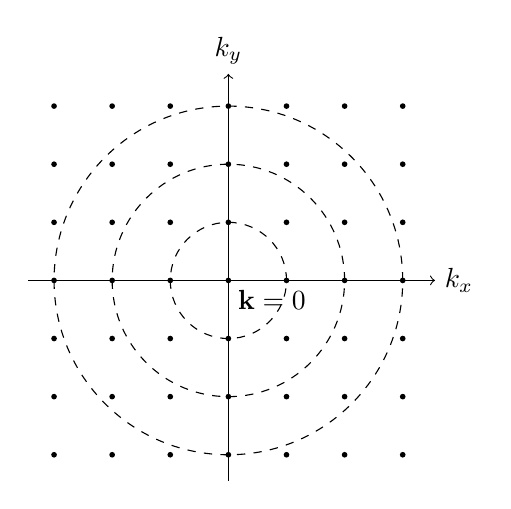
\begin{tikzpicture}[scale=0.82]
\draw[->] (-3.1,0) -- (3.2,0) node[right] {$k_x$};
\draw[->] (0,-3.1) -- (0,3.2) node[above] {$k_y$};
\draw[dashed] (0,0) circle (0.9);
\draw[dashed] (0,0) circle (1.8);
\draw[dashed] (0,0) circle (2.7);
\foreach \x in {-3,-2,-1,0,1,2,3}{
  \foreach \y in {-3,-2,-1,0,1,2,3}{
    \fill (0.9*\x,0.9*\y) circle (1.25pt);
  }
}
\node[below right] at (0,0) {$\mathbf{k}=0$};
\end{tikzpicture}
\caption{Estados discretos de momento y capas de energía constante para partículas en una caja periódica finita.}
\end{figure}

Para una partícula no relativista,
\begin{equation}
E_{\mathbf{k}}=\frac{\mathbf{k}^2}{2m},
\end{equation}
por lo que el estado de menor energía es \(\mathbf{k}=0\). Introduzcamos \(N\) bosones idénticos en la caja y busquemos el estado fundamental de muchas partículas. El primer bosón ocupa el estado de momento cero. El segundo puede ocupar ese mismo estado, al igual que el tercero y todos los siguientes. Así, los \(N\) bosones ocupan \(\mathbf{k}=0\).

Esto es un condensado de bosones: un gran número de partículas idénticas que ocupan el mismo estado de una partícula, aquí el estado de menor energía. La función de onda de momento cero es constante en el espacio y se extiende por toda la caja. No localiza ningún bosón en una posición determinada; por consiguiente, la posición de cada bosón es incierta. Cuando la ocupación se vuelve grande, la función de onda común genera una amplitud de campo macroscópica, y el campo se comporta cada vez más como un campo clásico.

El estado fundamental fermiónico es completamente distinto. Por el momento, ignoremos el espín, de modo que cada punto de momento represente un estado disponible. El primer fermión ocupa \(\mathbf{k}=0\), pero un segundo fermión idéntico no puede ocupar ese mismo estado. Las partículas siguientes deben ocupar la siguiente capa de menor energía. En un dibujo bidimensional hay cuatro puntos de red no nulos más próximos, todos con la misma energía; en tres dimensiones hay seis. Una vez ocupados esos estados, las partículas adicionales deben entrar en capas sucesivas.

Como la energía es proporcional al cuadrado de la distancia al origen en el espacio de momentos, minimizar la energía total equivale a llenar los puntos ocupados lo más cerca posible de \(\mathbf{k}=0\), hasta donde lo permita la exclusión. Con muchos fermiones, la región ocupada se aproxima a una esfera. Su frontera es la superficie de Fermi, su interior es el mar de Fermi, y toda la región llena es la esfera de Fermi. A volumen finito, la frontera es ligeramente irregular porque los puntos disponibles forman una red, pero este detalle se vuelve despreciable en un sistema grande.

\begin{figure}
\centering
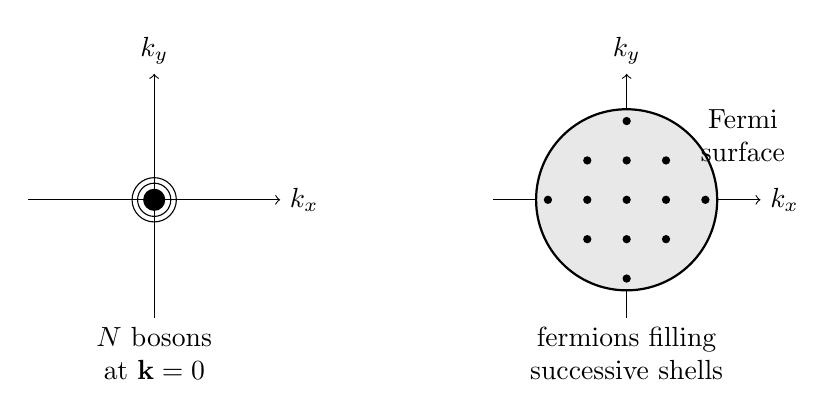
\begin{tikzpicture}[scale=1.0]
\begin{scope}[xshift=-3.0cm]
\draw[->] (-1.6,0) -- (1.6,0) node[right] {$k_x$};
\draw[->] (0,-1.5) -- (0,1.6) node[above] {$k_y$};
\fill (0,0) circle (4pt);
\draw (0,0) circle (6pt);
\draw (0,0) circle (8pt);
\node[align=center] at (0,-1.95) {$N$ bosons\\at $\mathbf{k}=0$};
\end{scope}
\begin{scope}[xshift=3.0cm]
\draw[->] (-1.7,0) -- (1.7,0) node[right] {$k_x$};
\draw[->] (0,-1.5) -- (0,1.6) node[above] {$k_y$};
\fill[gray!18] (0,0) circle (1.15);
\draw[thick] (0,0) circle (1.15);
\fill (0,0) circle (1.5pt);
\fill (0.5,0) circle (1.5pt);
\fill (-0.5,0) circle (1.5pt);
\fill (0,0.5) circle (1.5pt);
\fill (0,-0.5) circle (1.5pt);
\fill (0.5,0.5) circle (1.5pt);
\fill (0.5,-0.5) circle (1.5pt);
\fill (-0.5,0.5) circle (1.5pt);
\fill (-0.5,-0.5) circle (1.5pt);
\fill (1,0) circle (1.5pt);
\fill (-1,0) circle (1.5pt);
\fill (0,1) circle (1.5pt);
\fill (0,-1) circle (1.5pt);
\node[right,align=center] at (0.82,0.82) {Fermi\\surface};
\node[align=center] at (0,-1.95) {fermions filling\\successive shells};
\end{scope}
\end{tikzpicture}
\caption{Los bosones se condensan en el estado de momento cero, mientras que los fermiones van llenando los estados de momento hacia afuera hasta llegar a una superficie de Fermi.}
\end{figure}

El estado fundamental fermiónico tiene mucha más energía que el estado fundamental bosónico correspondiente. Todos los bosones pueden permanecer con momento cero, pero la mayoría de los fermiones se ven obligados a ocupar estados de momento no nulo. Al añadir más fermiones, aumenta el momento máximo ocupado. Además, una capa de gran momento contiene más puntos de red que una capa cercana al origen. Por ello, una esfera de Fermi grande contiene muchas partículas con momentos considerables y solo unas pocas en los estados de menor momento.

El contraste también se observa en los estados excitados. En el caso de los bosones, la primera excitación se obtiene sacando cualquier bosón del condensado y colocándolo en un estado excitado de una partícula:
\begin{equation}
(N,0,0,\ldots)\longrightarrow (N-1,1,0,\ldots).
\end{equation}
No importa cuál de los bosones se desplace: las partículas son idénticas. Las excitaciones de mayor energía pueden producirse de varias maneras. Según la separación entre niveles, se puede colocar un bosón en un nivel superior o dos bosones en el primer nivel excitado. Excitar el sistema bosónico significa promover partículas del condensado a estados de mayor energía.

En el caso de los fermiones, ninguna partícula puede trasladarse a otro punto dentro de la esfera de Fermi llena, porque todos esos puntos ya están ocupados. Es posible tomar un fermión del interior profundo del mar y colocarlo por encima de la superficie, pero eso requiere mucha energía. La excitación de menor energía consiste en tomar un fermión de justo dentro de la superficie de Fermi y trasladarlo a un estado desocupado justo fuera de ella. El electrón promovido tiene una energía apenas superior a la de la superficie, y el estado vacante que deja atrás está apenas por debajo de ella.

\begin{figure}
\centering
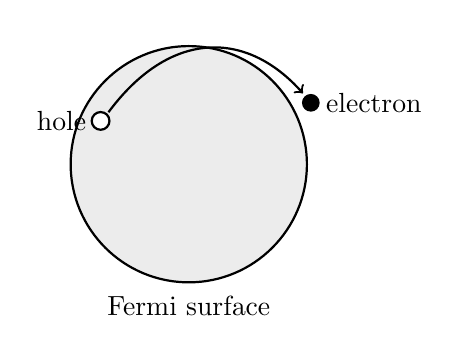
\begin{tikzpicture}[scale=1.0]
\fill[gray!15] (0,0) circle (1.5);
\draw[thick] (0,0) circle (1.5);
\draw[fill=white,thick] (-1.12,0.55) circle (3.2pt);
\fill (1.55,0.78) circle (3.2pt);
\draw[->,thick] (-1.02,0.66) .. controls (-0.25,1.7) and (0.72,1.72) .. (1.45,0.9);
\node[left] at (-1.18,0.55) {hole};
\node[right] at (1.62,0.78) {electron};
\node[below] at (0,-1.55) {Fermi surface};
\end{tikzpicture}
\caption{Una excitación fermiónica de baja energía promueve un electrón a través de la superficie de Fermi y deja un hueco.}
\end{figure}

\section{Huecos y excitaciones de baja energía}

Para concretar la carga del hueco, imaginemos que la caja contiene una carga positiva distribuida uniformemente por su volumen. En la materia, esa carga positiva proviene en última instancia de los protones de los núcleos, pero la distribución uniforme simplifica el modelo. Añadamos suficientes electrones para neutralizar el fondo. En el estado fundamental, esos electrones llenan la esfera de Fermi.

Promover un electrón desde debajo hasta encima de la superficie de Fermi no cambia la carga total de la caja. Crea un electrón con carga negativa por encima de la superficie y deja una carga negativa faltante por debajo. Por tanto, la ausencia del electrón puede tratarse como una excitación con carga positiva: un hueco.

\begin{classroomqa}
\lecturetimestamp{01:31:38}
\audiencequestion{¿Tiene energía negativa un hueco situado por debajo de la superficie de Fermi?}
\lecturerresponse{No. Un hueco es una excitación por encima del estado fundamental de muchos cuerpos, así que su energía de excitación es positiva. Quitar un electrón ocupado por debajo de la superficie de Fermi requiere una cantidad positiva de energía cuando las energías se miden con respecto a esa superficie.}
\end{classroomqa}

Sea \(\varepsilon<\varepsilon_F\) la energía del electrón extraído y \(\varepsilon'>\varepsilon_F\) la del electrón promovido. La energía suministrada puede descomponerse en dos distancias positivas respecto de la superficie de Fermi.\footnote{Los dos intervalos se indican por separado; la igualdad compacta que se muestra aquí es la reconstrucción algebraicamente equivalente.}
\begin{equation}
\Delta E
=\varepsilon'-\varepsilon
=(\varepsilon'-\varepsilon_F)+(\varepsilon_F-\varepsilon).
\end{equation}
La primera contribución se asigna de manera natural al electrón por encima de la superficie de Fermi, mientras que la segunda se asigna al hueco por debajo de ella:
\begin{equation}
E_{\mathrm{electron}}=\varepsilon'-\varepsilon_F>0,
\qquad
E_{\mathrm{hole}}=\varepsilon_F-\varepsilon>0.
\end{equation}
El electrón tiene carga negativa y el hueco tiene carga positiva.

Más tarde, un electrón por encima de la superficie de Fermi puede caer en un hueco disponible. Entonces su energía disminuye, por lo que la radiación debe llevarse la energía liberada. El suceso puede describirse como la caída de un electrón a un estado inferior desocupado, con emisión de uno o más fotones. De manera equivalente, puede decirse que un electrón y un hueco se aniquilan y producen radiación. El hueco no es un constituyente fundamental adicional de la caja; es una ausencia en el estado lleno de muchos electrones. Aun así, su energía y su carga hacen útil tratarlo como una excitación de tipo corpuscular.

\begin{classroomqa}
\lecturetimestamp{01:36:52}
\audiencequestion{¿Promover un electrón significa trasladarlo de un punto a otro de la red en el espacio de momentos?}
\lecturerresponse{Significa trasladar el electrón de un nivel de energía a otro. Para partículas libres en la caja, la red de momentos identifica esos niveles, pero la misma idea no depende de que exista una red en el espacio de momentos. En un átomo, la carga positiva está concentrada en el núcleo. Los electrones llenan los niveles atómicos disponibles de menor energía, y un fotón puede promover un electrón a un nivel excitado, dejando una vacante en el nivel del que salió. Esa vacante es el equivalente atómico de un hueco.}
\end{classroomqa}

En la caja, la absorción de un fotón convierte asimismo su energía en un electrón por encima de la superficie de Fermi y un hueco por debajo de ella. En un átomo, el mismo lenguaje describe el electrón excitado junto con la vacante que deja entre los niveles inferiores ocupados.

\begin{classroomqa}
\lecturetimestamp{01:39:16}
\audiencequestion{¿Puede un electrón situado en cualquier parte de la esfera de Fermi absorber un fotón de baja energía?}
\lecturerresponse{No. Si el electrón está en lo profundo del mar de Fermi, todos los estados cercanos ya están ocupados, y un fotón de baja energía no puede elevarlo hasta un estado desocupado por encima de la superficie. Solo los electrones suficientemente próximos a la superficie de Fermi tienen estados vacíos accesibles dentro del intervalo de energía del fotón. Un fotón con energía suficiente sí puede excitar un electrón desde las profundidades del mar.}
\end{classroomqa}

Por tanto, la sección eficaz de absorción a baja energía está determinada por la superficie del mar de Fermi, no por todo su volumen. Los electrones en lo profundo del mar no pueden efectuar transiciones pequeñas; los que están justo debajo de la superficie pueden pasar a estados justo por encima de ella.

\begin{classroomqa}
\lecturetimestamp{01:40:42}
\audiencequestion{¿Qué impide que los electrones interactúen directamente entre sí, sin un fotón incidente?}
\lecturerresponse{Nada. En este modelo sencillo se ignoran las interacciones electrón--electrón, porque incluirlas complica el modelo del mar de Fermi. En esta primera aproximación a un metal, se considera que su influencia efectiva es lo bastante débil como para poder ignorarla por lo general.}
\end{classroomqa}

\begin{classroomqa}
\lecturetimestamp{01:41:10}
\audiencequestion{¿Qué ocurre si un fotón tiene energía suficiente para excitar varios electrones?}
\lecturerresponse{En principio, es posible cualquier proceso compatible con las leyes de conservación. El fotón puede crear más de un par electrón--hueco: excitar dos electrones también deja dos huecos. Un proceso así crea más excitaciones y, en general, es menos probable que emplear la energía para excitar mucho más a un solo electrón.}
\end{classroomqa}

\begin{classroomqa}
\lecturetimestamp{01:42:06}
\audiencequestion{¿Pueden absorberse dos fotones a la vez cuando ninguno de ellos puede producir por sí solo la excitación?}
\lecturerresponse{Sí. La absorción es probabilística, y puede ocurrir un proceso de dos fotones cuando la energía combinada de ambos alcanza una excitación disponible, aunque cada uno por separado no alcance la energía requerida. Si la luz disponible tiene muy poca energía para alcanzar cualquier excitación permitida, atraviesa en gran medida el sistema.}
\end{classroomqa}

\editorialnote{Una breve discusión en este punto relaciona la radiación absorbida con el movimiento colectivo de los electrones, pero no se pueden recuperar sus detalles sustantivos. Solo es seguro afirmar que esa respuesta colectiva es más complicada que la descripción de una sola partícula--hueco.}

\begin{classroomqa}
\lecturetimestamp{01:43:49}
\audiencequestion{¿Por qué se dice que las interacciones electrón--electrón son débiles si todos los electrones tienen la misma carga negativa?}
\lecturerresponse{Los electrones están inmersos en el fondo positivo compensador. Ese fondo apantalla la carga de un electrón y reduce la interacción efectiva en este marco simplificado. La interacción no desaparece; para tratarla hay que tener en cuenta la respuesta de apantallamiento del medio.}
\end{classroomqa}

\begin{classroomqa}
\lecturetimestamp{01:44:41}
\audiencequestion{¿Se hablará del apantallamiento más adelante?}
\lecturerresponse{Sí. El apantallamiento es importante, pero se pospone hasta que se pueda tratar el sistema interactuante con más detalle.}
\end{classroomqa}

\section{Un mar fermiónico unidimensional y las antipartículas}

La construcción del hueco apunta hacia las antipartículas. La misma estructura lógica puede trasladarse de los electrones en la materia a un campo cuántico relativista y su vacío. La versión más sencilla emplea una dimensión espacial y un campo fermiónico sin masa \(\psi(x,t)\). En unidades en las que la velocidad de la luz es igual a uno, las dos relaciones de dispersión lineales posibles son
\begin{equation}
\omega=k,
\qquad\text{or}\qquad
\omega=-k.
\end{equation}
Consideraremos explícitamente la primera rama.

\editorialnote{El intercambio final alterna entre identificaciones de partículas incompatibles. El modelo seguro es un campo fermiónico de juguete sin masa, no especificado, en una dimensión espacial y restringido a una sola dirección de propagación.}

Para una onda plana
\begin{equation}
\psi(x,t)=e^{i(kx-\omega t)},
\end{equation}
las derivadas son
\begin{equation}
\frac{\partial\psi}{\partial t}=-i\omega\psi,
\qquad
\frac{\partial\psi}{\partial x}=ik\psi.
\end{equation}
Así, \(\omega=k\) equivale a la ecuación de campo de primer orden
\begin{equation}
\frac{\partial\psi}{\partial t}
=-\frac{\partial\psi}{\partial x}.
\end{equation}

\begin{figure}
\centering
\includegraphics[width=0.72\textwidth]{lecture_05_figure_05.png}
\caption{Inicio de la ecuación de campo de primer orden cuyas ondas planas satisfacen \(\omega=k\).}
\lectureframe{01:47:22}
\end{figure}

Cualquier perfil de la forma \(f(x-t)\) satisface esta ecuación y se propaga hacia la derecha. Al invertir el signo, se obtiene
\begin{equation}
\frac{\partial\psi}{\partial t}
=+\frac{\partial\psi}{\partial x},
\end{equation}
cuyos perfiles \(f(x+t)\) se propagan hacia la izquierda. Cada una de las ecuaciones de primer orden selecciona una sola dirección de movimiento. Supongamos que el campo es fermiónico y, para el argumento del hueco, que sus partículas tienen carga eléctrica.

La rama \(\omega=k\) presenta una dificultad inmediata. El número de onda \(k\) puede ser negativo y, por tanto, también puede serlo \(\omega\). Como \(\omega\) es la energía en estas unidades, el espectro lineal contiene estados de energía tanto positiva como negativa:
\begin{equation}
E=\omega=k.
\end{equation}

\begin{figure}
\centering
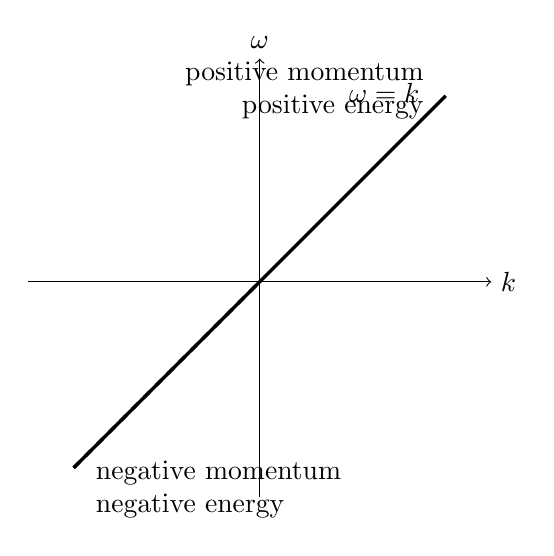
\begin{tikzpicture}[scale=1.05]
\draw[->] (-2.8,0) -- (2.8,0) node[right] {$k$};
\draw[->] (0,-2.6) -- (0,2.7) node[above] {$\omega$};
\draw[very thick] (-2.25,-2.25) -- (2.25,2.25);
\draw[very thick,dashed] (-2.25,-2.25) -- (0,0);
\node[above left] at (2.05,2.05) {$\omega=k$};
\node[below right,align=left] at (-2.1,-2.05) {negative momentum\\negative energy};
\node[above left,align=right] at (2.1,1.85) {positive momentum\\positive energy};
\end{tikzpicture}
\caption{El espectro de una sola rama \(\omega=k\), cuya mitad de energía negativa corresponde a \(k<0\).}
\end{figure}

Un vacío ordinario y vacío no puede ser el estado fundamental de una teoría así. Un fermión de energía positiva podría emitir un fotón y caer a un estado inferior. Nada le impediría detenerse en cero: podría seguir cayendo hacia estados de energía negativa, emitir aún más radiación y descender sin límite. La energía que pierde el fermión aparecería en el campo de radiación. Por tanto, un espectro no acotado inferiormente no tiene un vacío ordinario estable.

El principio de exclusión de los fermiones ofrece otro punto de partida. Llenemos con un fermión cada estado de una partícula de energía negativa, hasta llegar a la energía cero. Ningún otro fermión puede caer en esos estados porque ya están ocupados. Es imposible añadir otro fermión de energía negativa, mientras que añadir uno de energía positiva aumenta la energía. Por tanto, el mar de energía negativa completamente lleno puede tomarse como el estado fundamental de muchos cuerpos y llamarse vacío.

\begin{figure}
\centering
\resizebox{\linewidth}{!}{%
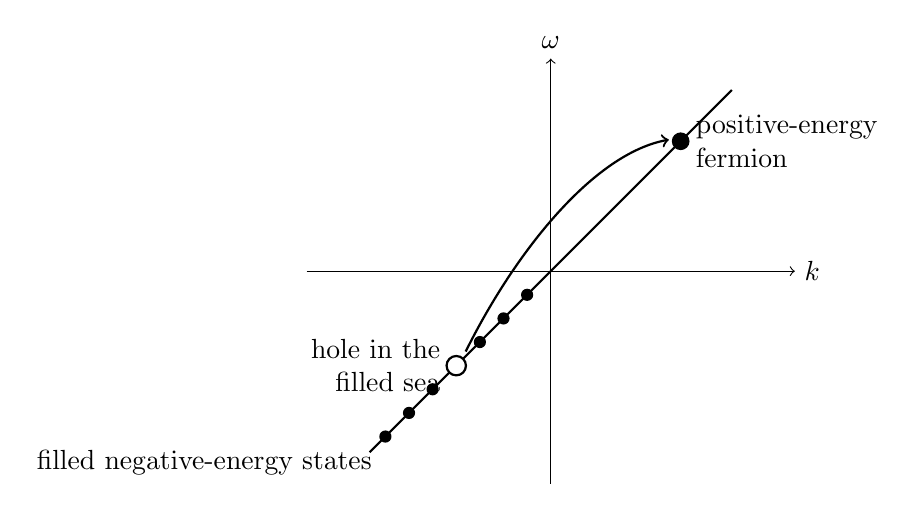
\begin{tikzpicture}[scale=1.0]
\draw[->] (-3.1,0) -- (3.1,0) node[right] {$k$};
\draw[->] (0,-2.7) -- (0,2.7) node[above] {$\omega$};
\draw[thick] (-2.3,-2.3) -- (2.3,2.3);
\foreach \p in {-2.1,-1.8,-1.5,-1.2,-0.9,-0.6,-0.3}{
  \fill (\p,\p) circle (2.2pt);
}
\draw[fill=white,thick] (-1.2,-1.2) circle (3.5pt);
\fill (1.65,1.65) circle (3.2pt);
\draw[->,thick] (-1.08,-1.02) .. controls (-0.45,0.25) and (0.55,1.5) .. (1.5,1.67);
\node[left,align=right] at (-1.28,-1.2) {hole in the\\filled sea};
\node[right,align=left] at (1.72,1.65) {positive-energy\\fermion};
\node[below left] at (-2.15,-2.15) {filled negative-energy states};
\end{tikzpicture}%
}
\caption{El mar de energía negativa lleno y una excitación formada al promover un fermión a energía positiva.}
\end{figure}

La excitación más sencilla consiste en extraer un fermión del mar de energía negativa y colocarlo en un estado de energía positiva. El fermión promovido es una partícula ordinaria de energía positiva. La vacante que queda en el mar es una segunda excitación: un hueco. Si el fermión extraído tiene carga negativa, el hueco tiene carga positiva.

En este ejemplo de una sola rama, el hueco también tiene momento positivo. Si el fermión ausente ocupaba un estado de momento \(k_-<0\), al extraerlo el momento total cambia en
\begin{equation}
p_{\mathrm{hole}}=-k_->0.
\end{equation}
Se trata, por tanto, de un déficit de momento negativo. Así, la excitación consta de un fermión de energía positiva y carga negativa, y de un hueco de energía positiva y carga positiva. Ambos tienen momento positivo y, en la rama \(\omega=k\), ambos se propagan hacia la derecha.

En la teoría completa del electrón, el hueco de carga positiva es el positrón. Dirac consideró inicialmente identificar el hueco con el protón. Esta construcción exige que una partícula y su antipartícula tengan la misma masa. El hueco es una partícula distinta, con la masa del electrón y carga eléctrica opuesta. Esta es la interpretación básica de partícula--antipartícula a la que condujo el espectro de energía negativa.

La misma solución no se puede aplicar a los bosones. Un estado bosónico admite un número arbitrario de partículas, así que no hay forma de llenar un nivel de energía negativa una sola vez e impedir que se ocupe más. Siempre se podrían añadir más bosones a ese nivel y reducir la energía una y otra vez:
\begin{equation}
\begin{aligned}
\text{fermionic mode: }&n=0\ \text{or}\ 1,\\
\text{bosonic mode: }&n=0,1,2,\ldots .
\end{aligned}
\end{equation}
El sistema bosónico propuesto seguiría sin tener estado fundamental. En esta construcción elemental, la estabilidad del mar lleno depende precisamente del principio de exclusión de los fermiones.

Esta ecuación unidimensional es solo una versión de juguete de la ecuación de Dirac. Su campo no tiene masa, se mueve a la velocidad de la luz y se propaga en una sola dirección. Una ecuación de Dirac más completa debe incorporar las direcciones de movimiento que faltan y el resto de la estructura de las partículas relativistas. Se posponen esa ecuación más completa y el tratamiento de las antipartículas de los campos bosónicos.
